%! Author = wolfram_e_laube
%! Date = 06.05.24

\item[(a)]
\subsection{Task (a): Real and Imaginary Parts of $X(f)$}

\subsubsection{Problem Statement}
Visualize the real and imaginary components of the frequency spectrum $X(f)$, given its magnitude $|X(f)|$ and phase $\phi_x(f)$, and discuss the implications of these components in signal processing.

\subsubsection{Mathematical Formulation}
Given:
\begin{itemize}
    \item \textbf{Magnitude $|X(f)|$:}
    \[
    |X(f)| =
    \begin{cases}
    A & \text{if } -5 \leq f < -1 \text{ or } 1 < f \leq 5 \\
    A(1 + f) & \text{if } -1 \leq f < 0 \\
    A(1 - f) & \text{if } 0 \leq f \leq 1 \\
    0 & \text{otherwise}
    \end{cases}
    \]

    \item \textbf{Phase $\phi_x(f)$:}
    \[
    \phi_x(f) =
    \begin{cases}
    \frac{\pi}{2} & \text{if } -5 \leq f < 0 \\
    -\frac{\pi}{2} & \text{if } 0 < f \leq 5 \\
    0 & \text{otherwise}
    \end{cases}
    \]
\end{itemize}

Using Euler's formula:
\[
X(f) = |X(f)| \cdot e^{i \phi_x(f)}
\]
\[
\text{Re}\{X(f)\} = |X(f)| \cos(\phi_x(f))
\]
\[
\text{Im}\{X(f)\} = |X(f)| \sin(\phi_x(f))
\]

\subsubsection{Discussion}
The real part $\text{Re}\{X(f)\}$ is zero for all $f$, reflecting the phase shifts of $\frac{\pi}{2}$ and $-\frac{\pi}{2}$. The imaginary part $\text{Im}\{X(f)\}$ shows variations with $f$, mirroring the magnitude adjustments and the sinusoidal phase behavior.

\begin{figure}[h]
    \centering
    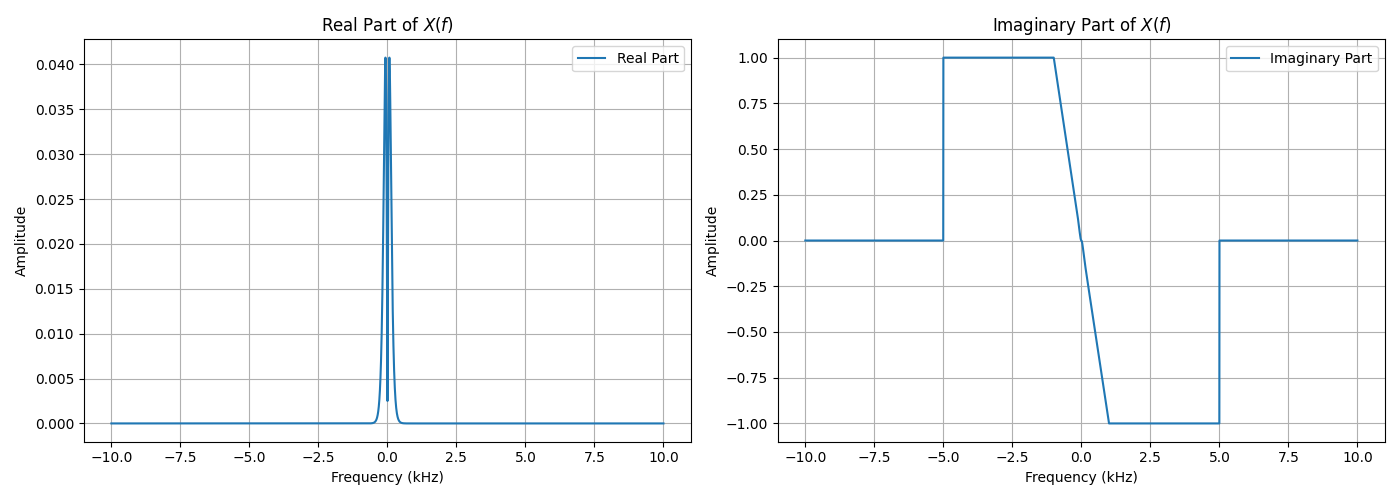
\includegraphics[width=0.49\textwidth]{fig/ex2_a_plot}
    \caption{Real and Imaginary Parts of $X(f)$}
    \label{fig:ex2_a_plot}
\end{figure}
